% Repository:  https://github.com/chiehrosswang/TRB_LaTeX_tex
%
% Transportation Research Board conference paper template
% version 4.0 Lite (updates made to be compatible in Overleaf and ShareLaTeX)
% 
% When numbered option is activated, lines are numbered.
\documentclass[numbered]{trbunofficial}
\usepackage{graphicx}
\usepackage{booktabs}
\usepackage{amsmath}
\usepackage{color,soul}
%\usepackage{caption}
\usepackage{subcaption}

% \usepackage[colorlinks=true,linkcolor=blue,citecolor=blue]{hyperref}
% For TRB version hide links
\usepackage[hidelinks]{hyperref}
\def\equationautorefname~#1\null{Equation #1\null}

% Put here what will go to headers as author
\AuthorHeaders{Lin, Wang, and Chen}
\title{Optimizing Routing of Mobile Retroreflectivity Units for Pavement Marking Performance Assessment}

% TODO: add macros for easier formatting of \author.
\author{%
  \textbf{Yu-Chun Lin}\\
  Department of Civil Engineering, National Taiwan University\\
  Taipei, Taiwan 106\\
  Email: \href{r06521515@ntu.edu.tw}{r06521515@ntu.edu.tw}\\
  \hfill\break% this is a way to add line numbering on empty line
  \textbf{Chieh (Ross) Wang, Ph.D.}\\
  Energy and Transportation Science Division, Oak Ridge National Laboratory (ORNL)\\
  Oak Ridge, TN 37831\\
  Email: \href{mailto:cwang@ornl.gov}{cwang@ornl.gov}\\
  ORCID: \href{https://orcid.org/0000-0001-8073-7683}{0000-0001-8073-7683}\\
  \hfill\break%
  \textbf{Albert Y. Chen, Ph.D., Corresponding Author}\\
  Department of Civil Engineering, National Taiwan University\\
  Taipei, Taiwan 106\\
  Email: \href{albertchen@ntu.edu.tw}{albertchen@ntu.edu.tw}\\
  ORCID: \href{https://orcid.org/0000-0001-6702-9834}{0000-0001-6702-9834}\\
}

% If necessary modify the number of words per table or figure default is set to
% 250 words per table
% \WordsPerTable{250}

% If words are counted manually, put that number here. This does not include
% figures and tables. This can also be used to avoid problems with texcount
% program i.e. if one does not have it installed.
% \TotalWords{200}

\begin{document}
\maketitle

\section{Abstract}
Evaluation of pavement marking visibility/retroreflectivity has advanced from visual and/or manual inspections, which can be unsafe, subjective, and time-consuming, to mobile assessments using vehicle-mounted devices, allowing transportation agencies to collect retroreflectivity data at a large scale in a safer and more efficient manner. However, cost-effectively routing and operating these mobile retroreflectivity units (MRUs) at such a large scale can be a unique challenge. This study proposes a vehicle routing problem (VRP) based model to optimize the routing of MRUs. The model takes into account the costs of daily and weekly operations of MRUs, including remounting the device from one side of the vehicle to the other and traveling between tasks.  A case study is conducted using the proposed VRP-based model to optimally route MRUs to tackle 15 to 30 tasks and the solutions are compared with actual routing schedules of the MRU team of the Florida Department of Transportation in the most recent data collection cycle. The average savings from the proposed model is 36.7\% for the MRU vehicles' travel distance, and 48.5\% of the model objective value. The proposed methodology can effectively reduce the operational cost calculated based on the objective function and the total distance traveled.

\hfill\break%
\noindent\textit{Keywords}: Vehicle Routing Problem, Pavement Marking Performance, Retroreflectivity, Mobile Retroreflectivity Units
\newpage

\section{Introduction}
Longitudinal pavement markings, referred to as lane markings hereinafter, are an important type of traffic control devices that is crucial to roadway safety. Periodically assessing lane marking conditions, i.e., visibility and retroreflectivity, ensures the proper function and performance of lane markings. Traditionally, lane marking assessment involves visual windshield surveys and manual data collection using handheld devices, which can be subjective, small scale, time-consuming, and unsafe. 

Recent development and advances in the Mobile Retroreflectivity Unit (MRU) technology -- a laser-based equipment that can be mounted on a vehicle while measuring pavement marking retroreflectivity at highway speeds -- have provided opportunities for state and local transportation agencies to collect pavement marking retroreflectivity data efficiently on a large scale.  State departments of transportation (DOTs), such as the Florida Department of Transportation (FDOT), have conducted annual or biannual state-wide pavement marking condition evaluation using MRUs and developed a Pavement Marking Management System (PMMS) that provides detailed retroreflectivity data for internal and external users, such as maintenance engineers and striping contractors, to make data-driven decisions \cite{Choubane2018,pmms}.  

Often, state DOTs rely on field operators and/or contractors to artificially plan the routes and carry out the testing.  However, collection of state-wide pavement marking data on all state-maintained roadways on an annual basis can be a challenging task.  Various factors (e.g., traffic, fog, wet weather, hurricanes, snow, debris on the road, equipment and vehicle maintenance, etc.) can significantly affect the testing schedule.  To ensure there is enough buffer time to deal with these external factors that are not of anyone's control, there is a need, therefore, to optimize the operational scheduling, which can be governed by the data collection team.

One way of minimizing the data collection effort is to formulate the daily and weekly routing plans as a mathematical problem and solve it using optimization techniques.  In this context, each MRU testing task can be considered as a node of a network and the distance between a pair of nodes forms a link of the network.  Vehicle routing problem (VRP) models can be used for solving the sequence of the nodes being visited and the links being traveled on, which then ensures the optimal solution of the objective under various constraints. If there is a complete network, we can form the VRP model and the testing schedule can be optimized.  Unlike many other VRPs, the objective of the VRP for MRU operations not only considers minimal distance travelled, but also should take into account the temporal constraints (e.g., number of operating hours per day, number of operating days per week) as well as equipment configuration and reconfiguration cost.  These aspects of the objective make the VRP for MRU operations unique and more complicated.

The purpose of this study is to formulate an integer program (IP) for optimizing lane marking assessment scheduling and provide a structured way to generate efficient assessment routing plans.  The paper is structured as follows: The second section gives an overview of the state-of-the-practice lane marking assessment and VRP models; the third section describes the detailed mathematical formulation of the unique MRU routing problem; the fourth section presents a case study in which historical FDOT scheduling certain number of tasks were compared with the optimized scheduling of the same tasks solved by the proposed methodology; finally, the fifth section concludes this paper and discusses potential future research.


\section{Literature Review}
\subsection{Lane Marking Assessment}
Lane markings are important traffic control devices that provide guidance to road users and are a crucial element of traffic safety. The visibility of pavement markings, in terms of the presence, contrast, and retroreflectivity, affects how well humans and machines can see the lane.  To ensure markings continue to serve their intended functions adequately, routine evaluation, monitoring, and timely maintenance are critical \cite{Choubane2018}. Traditional methods for assessing pavement marking conditions are through handheld devices and visual inspections. However, use of such methods can be ineffective and dangerous \cite{Holzschuher2010}. Recent advances in the Mobile Retroreflectivity Unit (MRU) -- a vehicle equipped with a mobile retroreflectometer capable of measuring pavement marking retroreflectivity at highway speed, provide a feasible means for transportation agencies to efficiently and safely collect marking retroreflectivity data at a large scale. The safety and efficiency advantages of MRUs have drawn attentions among transportation agencies and contractors, many of which have started utilizing MRUs to measure retroreflectivity at various scales. 

With the aforementioned advantages of MRUs, nevertheless, there are several limitations and factors that can affect the data collection schedule.  First, MRUs are usually required to be operated only on dry surfaces during dry weather conditions.  Second, debris on the road, winter weather treatments, pavement preventive treatments, and road constructions prevent the markings to be properly measured.  Third, different line types may require the MRU to be mounted differently and reconfiguring the MRU takes time.  In order to measure different types of lane markings, depending on the design of the MRUs, most MRUs currently available on the market need to be mounted on one side of the vehicle. As depicted in \textbf{Figure \ref{fig:1}}, the MRU needs to be mounted on the driver side of the vehicle when testing Type 1 lines (yellow center lines) and on the passenger side of the vehicle for testing Type 3 lines (white edge lines). Forth, routine laboratory and field calibration are crucial to the precision of the device.  Lack of calibration or poor mounting procedures can lead to inaccurate measurements. As \citep{Choubane2013} pointed out, MRUs are fairly sensitive instruments and if they are not properly calibrated and routinely inspected, accuracy and precision of the tests will be affected. These limitations and challenges make the routing of MRU operations a unique and interesting problem that has not been extensively studied.

\begin{figure}[!ht]
    \centering
    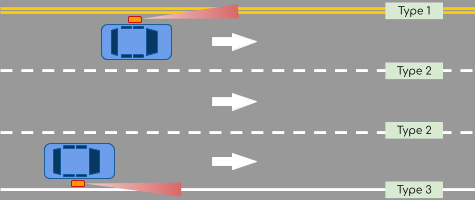
\includegraphics[width=0.8\textwidth]{figures/fig1.png}
    \caption{Types of lane markings and MRU mounting illustration.}
    \label{fig:1}
\end{figure}

\subsection{Vehicle Routing Problem}
The Vehicle Routing Problem (VRP) is an extension of the Traveling Salesman Problem (TSP) \cite{Dantzig2008}, which is a classical problem for routing. The VRP seeks best routes that services a number of customers with a fleet of vehicles from depots. The objective of the VRP usually minimizes transportation costs (traveling time or distance). \citep{Kulkarni1985} purposed requirements of the VRP model, including (1) meeting all customers' demands; (2) posing certain restrictions on the number of consumers/nodes assigned to each vehicle; and (3) limiting the total travel cost per vehicle and the service capacity with limits for each vehicle. Moreover, there are two assumptions for VRP. First, the maximum demand at a location $i$ is less than the minimum capacity of a vehicle, and the second is whenever a customer $i$ is serviced, the demand at $i$ is fulfilled.

A basic VRP restricts the relationship between vehicles, nodes and arcs. Constraints in the VRP must: (1) ensure a vehicle only visits and leaves one customer once; (2) ensure if a vehicle visits one customer, it must leave the same customer; (3) guarantee all routes start and end at a depot; (4)  limit  the capacity and maximum cost of each vehicle; and (5) eliminate subtours.

The complexity of reality brings about extensions of VRP in academic research and practical applications. For example, there are VRPs with time windows (VRPTW), time dependent VRPs (TDVRP) \cite{10.2307/25768538}, fleet size and mix VRPs (FSVRP), VRPs with multiple use of vehicle (VRPM), the two-echelon capacitated VRP \cite{Perboli2011}, and many more variations. 

When solving VRPs in a larger scale a solution algorithm is usually needed. \citep{Gracia2014} apply VRP to address the biomass collection problem \cite{Gracia2014}. Since the various machines interact with each other during the harvesting process, the path and work order of the different machines becomes important. Meta heuristics such as the Genetic algorithms (GA) and local search methods are used to obtain solutions \cite{YueqinZhang2008}.

VRP has also been proposed for road inspection work \cite{wang2013}, waste management \cite{Sahoo:2005:ROW:1052709.1052730}, city logistics planning \cite{Crainic:2009:MEP:1656425.1656429}, equipment allocation \cite{Chen2011}, in-building emergency rescue \cite{Chen2016}, and many more. There are in-depth reviews of VRP's theory and applications \cite{Laporte:2009:FYV:1656425.1656427,PILLAC20131}.

\subsection{Summary}
As more and more transportation agencies start using MRUs to collect retroreflectivity data at a large scale, being able to efficiently operating and routing the MRUs becomes more important from the operations and management standpoints.  The VRP has been extended to handle many similar applications in logistics, construction, and maintenance. The lane marking assessment problem can be described through a network of nodes and links, and planning of the MRU testing schedule can be formulated as a VRP problem.

\section{Methodology}
This section describes the formulation of a VRP-based model for routing MRU vehicles conducting lane marking assessments. The objective contains the operational cost, reconfiguration cost and travel cost. The goal of the model is to provide a system-wise assessment schedule.


\subsection{Nomenclature}
In the following are the definition of the variables, sets, and parameters used in the proposed model. 

\subsubsection{Variables}
\begin{itemize}
    \item $X_{odvtws}$ is non-negative binary variable that indicating whether link of node $o$ to node $d$ uses vehicle $v$ in period $t$, workday $w$ with tool installed in side $s$ is functional or not. 1 means link is used and 0 otherwise.
    \item $Y_t$ is non-negative binary variable representing period $t$ is used or not.
    \item $Z_{tw}$ is binary variable representing period $t$, workday $w$ is used or not. 
    \item $U_n$ is non-negative variable for subtour elimination.
    \item $SN_{vtwns}$ is non-negative binary variable indicating whether vehicle $v$ operating in period $t$, workday $w$ changes installation type of test tool from other type to type $s$ or not. 1 means change side and 0 otherwise.
    \item $ST_{vtw}$ is non-negative variable indicating reconfiguration times of vehicle $v$ in period $t$, workday $w$.
    \item $Td$ is non-negative variable describing total travel distance.
\end{itemize}

\subsubsection{Sets}
\begin{itemize}
    \item $N$ is set of nodes expect depot, and $O$, $D$ are same meaning but for readability.
    \item $H$ is set of depot nodes
    \item $V$ is set of depot nodes
    \item $T$ is set of periods
    \item $W$ is set of workdays
    \item $S$ is set of configuration types.
\end{itemize}

\subsubsection{Parameters}
\begin{itemize}
\item $C_{od}$ is travel distance from node $o$ to node $d$
\item $B_{od}$ is speed limit of node $o$ to node $d$
\item $F$ is allowed working hours per period
\item $f$ is allowed working hours per working day
\item $\alpha$, $\beta$, $\gamma$, and $\delta$ are constant of variables in objective function  
\end{itemize}



\subsection{Problem Formulation}
The following are the objective function and constraints that compose the proposed model.

\begin{equation}\label{eq:1}
    \qquad  \min ~\alpha\sum_{t\in T}Y_{t}+\beta \sum_{w\in W}\sum_{t\in T} Z_{t w}+\gamma \sum_{w\in W}\sum_{t\in T}\sum_{v\in V} S T_{v t w}+\delta T d
\end{equation}
\\
Subject to\\
\begin{equation}
    \qquad 
    \displaystyle \sum_{s\in S} \sum_{w\in W} \sum_{t\in T} \sum_{v\in V} \sum_{d\in D\cup H} X_{o d v t w s}=1 \quad \forall o \in \mathrm{N}\label{eq:2}
\end{equation}

\begin{equation}
    \qquad 
    \sum_{s\in S} \sum_{w\in W} \sum_{t\in T} \sum_{v\in V} \sum_{o\in O\cup H} X_{o d v t w s}=1 \quad \forall d \in N \label{eq:3}
\end{equation}

\begin{equation}
    \qquad 
    \sum_{s\in S} \sum_{w\in W} \sum_{o\in O\cup H} X_{o n v t w s} = \sum_{s\in S} \sum_{w\in W} \sum_{d\in D\cup H} X_{n d v t w s} \quad \forall n \in N\cup H, v \in V, t \in T \label{eq:4}
\end{equation}
\begin{equation}
    \qquad 
    \sum_{s\in S} \sum_{w\in W} \sum_{o\in O} X_{o h v t w s} \leq 1 \quad \forall h \in H, v \in V, t \in T\label{eq:5}
\end{equation}
\begin{equation}
    \qquad 
    \sum_{s\in S} \sum_{w\in W} \sum_{d\in D} X_{h d v t w s} \leq 1 \quad \forall h \in H, v \in V, t \in T \label{eq:6}
\end{equation}
\begin{equation}
    \qquad 
    u_{o}-u_{d}+(N+H)\times \sum_{s\in S} \sum_{w\in W} \sum_{t\in T} \sum_{v\in V} x_{o d v t w s} \leq N+H-1 \quad \forall o,d \in N, o \neq d \label{eq:7}
\end{equation}
\begin{equation}
    \qquad 
    Y_{t} \geq X_{o d v t w s} \quad \forall o \in O, d \in D, v \in V, t \in T, w \in W, s \in S \label{eq:8}
\end{equation}
\begin{equation}
    \qquad 
    Z_{t w} \geq X_{o d v t w s} \quad \forall o \in O, d \in D, v \in V, t \in T, w \in W, s \in S \label{eq:9}
\end{equation}
\begin{equation}
    \qquad 
    \sum_{s\in S} \sum_{w\in W} \sum_{d\in D\cup H} \sum_{o\in O\cup H} \frac{C_{o d}}{B_{o d}} X_{o d v t w s} \leq F \quad \forall v \in V, t \in T \label{eq:10}
\end{equation}
\begin{equation}
    \qquad 
    \sum_{s\in S} \sum_{d\in D\cup H} \sum_{o\in O\cup H} \frac{C_{o d}}{B_{o d}} X_{o d v t w s} \leq f \quad \forall v \in V, t \in T, w \in W \label{eq:11}
\end{equation}
\begin{equation}
    \qquad 
    S N_{v t w n s} \geq \sum_{o\in O\cup H} X_{o n v t w s^{\prime}}+\sum_{D} X_{n d v t w s}-1 \quad \forall n \in N, v \in V, t \in T, w \in W, s,s^{\prime} \in S, s\neq s^{\prime} \label{eq:12}
\end{equation}
\begin{equation}
    \qquad 
    S T_{v t w} \geq \sum_{s\in S} \sum_{n\in N} S N_{v t w n s} \quad \forall v \in V, t \in T, w\in W \label{eq:13}
\end{equation}
\begin{equation}
    \qquad 
    T d \geq \sum_{s\in S} \sum_{w\in W} \sum_{t\in T} \sum_{v\in V} \sum_{d\in D\cup H} \sum_{o\in O\cup H} C_{o d}X_{o d v t w s} \label{eq:14}
\end{equation}
\begin{equation}
    \qquad 
    \sum_{s\in S} \sum_{w \in \mathrm{w}-\mathrm{end}} \sum_{d\in D\cup H} X_{n d v t w s} \geq \sum_{s\in S} \sum_{o\in O \cup H} X_{o n v t w s} \quad \forall n \in N, v \in V, t \in T, w \in W \label{eq:15}
\end{equation}
\begin{equation}
    \qquad 
    Y_{t+1} \leq Y_{t} \quad \forall t \in T-1 \label{eq:16}
\end{equation}
\begin{equation}
    \qquad 
    Z_{t(w-1)} \leq Z_{t w} \quad \forall t \in T, w\in W-1 \label{eq:17}
\end{equation}
\\
The objective function (\textbf{Equation~\ref{eq:1}}) is composed of the aforementioned costs with different given weights to evaluate the performance of assessment schedule. Operational cost represents the total time cost for finishing all tasks. Configuration cost is measured in time units for switching the mount side of the MRU. Travel cost is the sum of all travel distance (or time).
\textbf{Equations~\ref{eq:2}-\ref{eq:7}} are the basic VRP constraints. Test vehicles in each period are ensured to arrive and leave each node (expect at the depot node) once as enforced in \textbf{Equations~\ref{eq:2}} and \textbf{\ref{eq:3}}. \textbf{Equation~\ref{eq:4}} indicates flow conservation. Each vehicle can only leave the depot less than once as enforced in \textbf{Equation~\ref{eq:5}}. Based on \textbf{Equation~\ref{eq:4}}, \textbf{Equation~\ref{eq:6}} indicates the vehicle must come back to the depot if it has set out. \textbf{Equation~\ref{eq:7}} eliminates subtours.

This formulation considers practical conditions, including the test vehicles may need maintenance periodically, the operators will not drive vehicle during weekends, and the test vehicles are requested to return to the depot by the end of the week. The formulation uses operating hours in a period (week) to satisfy this request in \textbf{Equation~\ref{eq:10}}. \textbf{Equation~\ref{eq:11}} is another inequality for operating hours per workday. \textbf{Equation~\ref{eq:8}} and \textbf{\ref{eq:9}} calculate the total operating period and workday.

Tools installation or reconfiguration increase operating time. To avoid the assessment schedule with an inefficient plan, \textbf{Equation~\ref{eq:12}} indicates whether operators change configuration types in the node (i.e., if the vehicle enters node with the MRU mounted on one side of the vehicle but leaves with the MRU mounted on the other side, then the value of the right hand side in \textbf{Equation~\ref{eq:12}} becomes 1, and thus the left hand side variable will be more than 1). \textbf{Equation~\ref{eq:13}} calculates the total times of reconfiguration. 

\textbf{Equation~\ref{eq:14}} sums the total travel distance and the left hand side variable is for readability. The workdays in a period have time sequence, and \textbf{Equation~\ref{eq:15}} makes sue vehicles will not violate the workday sequence. For example, \textbf{Equation~\ref{eq:15}} means if the vehicle enters the node on workday $w$, the vehicle cannot visit remaining nodes on days before w of the same period anymore. 

\textbf{Equations~\ref{eq:16}} and \textbf{\ref{eq:17}} express time. \textbf{Equation~\ref{eq:16}} indicates if the previous period was not utilized for operation, then the following periods are not allowed. \textbf{Equation~\ref{eq:17}} has the same concept for workday instead of period. 


\section{Case Study}
In this section, the proposed methodology is applied to the Florida Department of Transportation (FDOT)'s MRU program. The program has a yearly schedule and there are inventory lane markings needed to be measured every year. The tasks of lane marking section are located throughout the entire Florida state.

For the implementation of the formulation, Python is chosen as the programming language and the mathematical programming solver Gurobi \cite{Gurobi} is utilized. The analysis is executed on a computer with 8GB 2,133 MHz LPDDR3 memory and a 2.3 GHz Intel Core i5 CPU.

\subsection{Nodes and Arcs}
To enable a VRP-based model, a network has been developed. In this study, the nodes of network are transformed from jobs (tasks) of the MRU program, as shown in \textbf{Figures \ref{fig:2-1} and \ref{fig:2-2}}. Each task represents a section of the road to be measured, which contains an origin mile point and a destination mile point. The origin point and destination point are converted into different nodes in the network, as shown in \textbf{Figure \ref{fig:2-2}}. With these nodes and the depot (i.e., the base station), there can be three types of arcs that connect these nodes:
\begin{enumerate}
    \item The arc of a task (blue dotted arrow in \textbf{Figure \ref{fig:2-3}}): This type of arcs connect the origin and destination nodes of the same task;
    \item Arcs between different tasks (blue solid arrow in \textbf{Figure \ref{fig:2-3}}): this type of arcs connects the destination node of a task to the origin node of another task; and
    \item Arcs between tasks and depot (black solid arrow in \textbf{Figure \ref{fig:2-3}}): this type of arcs connect the depot (i.e., base station) to the origin of tasks or from the destination of tasks. 
\end{enumerate}

Nodes will be visited according to arcs, which implies through the manipulation of arcs value, nodes of same
task are guaranteed to be visited in turn. \textbf{Figures \ref{fig:2-1}}, \textbf{\ref{fig:2-2}}, and \textbf{\ref{fig:2-3}} demonstrate design of the network.

Travel distance is used for arcs. There are two types of travel distance in this case. One is distance between different tasks, which is extracted from the Open Street Routing Machine (OSRM) API. The OSRM runs on OpenStreetMap data and provides the environment and API to request the distance between locations. The other is distance between nodes of same task, which is extracted from the given starting and ending mile points of each task.

\begin{figure}[!ht]
    \centering
    \begin{subfigure}[b]{0.31\textwidth}
    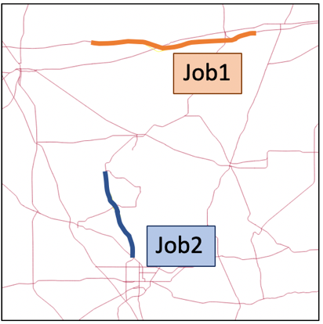
\includegraphics[width=\textwidth]{figures/fig2-1.PNG}
    \caption{Original}
    \label{fig:2-1}
    \end{subfigure}
    \begin{subfigure}[b]{0.31\textwidth}
    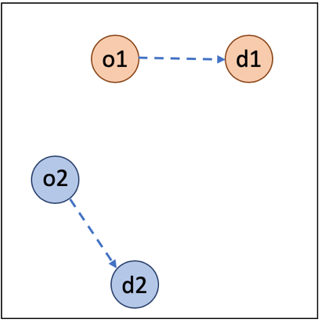
\includegraphics[width=\textwidth]{figures/fig2-2.PNG}
    \caption{Converted}
    \label{fig:2-2}
    \end{subfigure}
    \begin{subfigure}[b]{0.31\textwidth}
    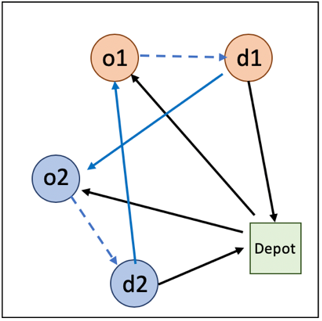
\includegraphics[width=\textwidth]{figures/fig2-3.PNG}
    \caption{Network}
    \label{fig:2-3}
    \end{subfigure}
    \caption{Conversion of the original tasks into the network for the optimization model.}
\end{figure}


\subsection{Settings of MRU program}
In the MRU program, there are two MRU vehicles for testing retroreflectivity of lane markings. Drivers depart from the depot on Monday and come back to the depot on Thursday, and all measure tasks need to be finished in 52 weeks. In correspondence with the model formulation, there are 52 periods and 4 workdays in each period in the MRU program. There are two types of configuration of MRUs. The retroreflectivity is measured by MRU vehicle in this case and tasks of lane marking are to be conducted with the MRU mounted on different sides. There will be a reconfiguration cost if the tasks need different types of equipment configuration.


\subsection{Results}
As a demonstration of the proposed model, tasks in Gilchrist county was conducted to verify the correctness of the model. In \textbf{Table \ref{tab:1}} the parameters and result of the model are listed. In this case, the 6 tasks in Gilchrist County, Florida can be optimally carried out by 1 MRU vehicle in 1 workday, and the total distance travelled, including testing distance and the distance in between tasks, was 306,538 m, which is about 192 miles.

\begin{table}[!ht]
\centering
\small
\caption{Model Validation using Gilchrist County Tasks}
\label{tab:1}
%\resizebox{0.8\textwidth}{!}{%
\begin{tabular}{@{}ll@{}}
\toprule
\small
%Case & 1 \\ \midrule
Tasks & 6 tasks in Gilchrist County \\
Constants ($\alpha~ ~\beta~ ~\gamma~ ~\delta$) & 6,000,000~ ~100,000~ ~50,000~ ~1\\
Operating cost & 1 vehicle operates in 1 week with 1 workday \\
Reconfiguration cost & 1 time of reconfiguration\\
Travel distance (m) & 306,538.616 \\
Solution time & 85.46s \\ 
\bottomrule
\end{tabular}%
%}
\end{table}



This study further used the historical schedule of the MRU program in the state of Florida for the 2018-2019 cycle as a benchmark for the case study. Execution sequence and the number of MRU vehicles utilized are recorded in the historical data set. 

The case is divided into scales of 15, 20, 25, and 30 tasks. We denote the results from the proposed model as ``Proposed'' in the following paragraphs. \textbf{Figure~\ref{fig:3}} depicts the geospatial distribution of tasks for the scale 30 case.

The history and Proposed results are depicted in \textbf{Tables \ref{tb:4} and \ref{tb:4-2}}. The distance value of history results is the sum of the driving distance of tasks in the historical order. However, the distances are calculated using the constructed network as previously described.  The vehicle value records the actual number of used MRU vehicles in the historical schedule. Reconfiguration records when the configuration type of the MRU changes.







The model of this study is aimed to improve the efficiency of the MRU operation schedule, including the reduction of the driving distance, the amount of MRU vehicle number and the reconfiguration time. 

In \textbf{Tables \ref{tb:4} and \ref{tb:4-2}}, we can see that the model of this study provides more efficient schedules. Tasks in all cases and scales can be finished in less driving distance, MRU vehicles and reconfiguration time. 


In \textbf{Table \ref{tb:5}}, the savings, i.e. the reduction in cost, from the proposed model in comparison to the actual task sequence in the case study is presented. The average savings from the proposed model for all cases listed in \textbf{Tables \ref{tb:4} and \ref{tb:4-2}} is 36.7\% for the MRU vehicles' travel distance, and 48.5\% in terms of the cost reduction of the objective value, based on \textbf{Equation~\ref{eq:1}}. 

We can expect if the model results are used for the State of Florida, the data collection of lane marking assessment can be reduced as high as 39.4\% in terms of traveling distance.


\begin{figure}[!ht]
    \centering
    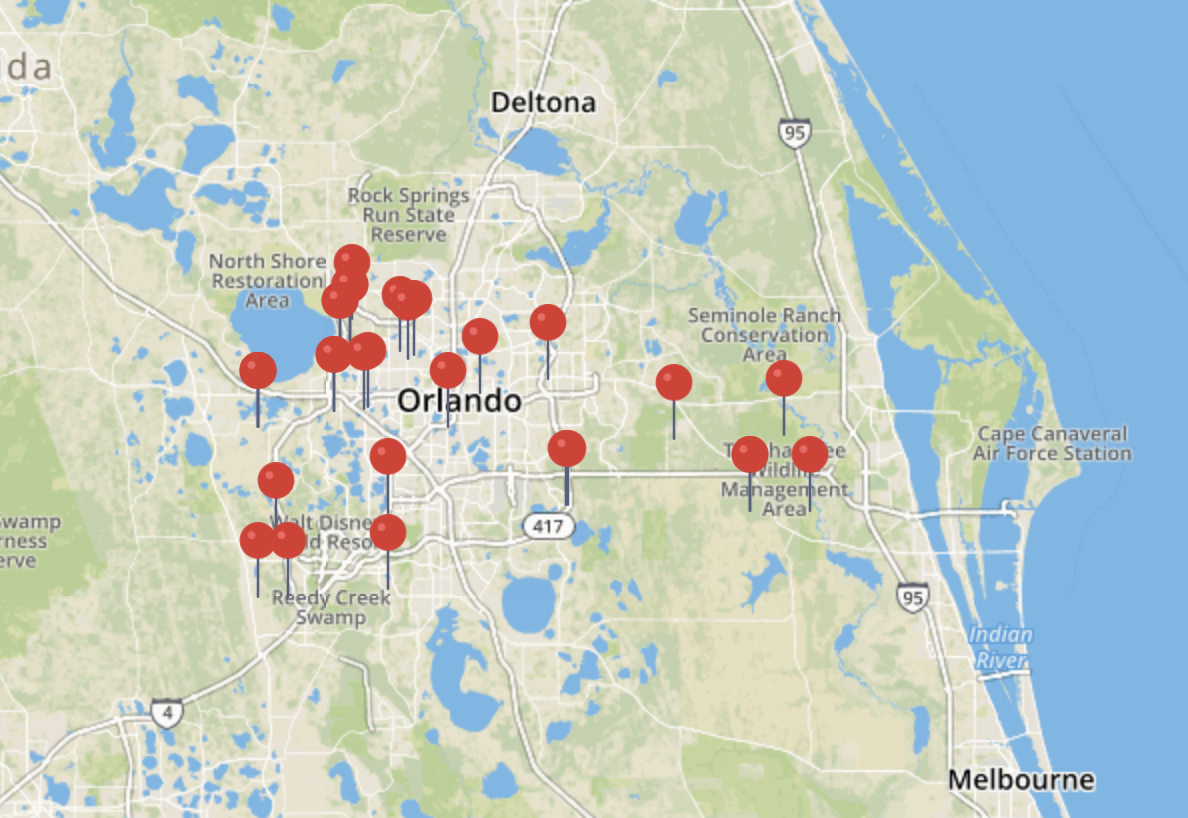
\includegraphics[width=0.8\textwidth]{figures/yuchun_map.png}
    \caption{Tasks of the Scale 30 case.}
    \label{fig:3}
\end{figure}


% table4
\begin{table}[!ht]
\small
\centering
\caption{Comparison of Results}\label{tb:4}
\begin{tabular}{ l rr rr }
\toprule 
{}&
\multicolumn{2}{ c }{15 tasks}&
\multicolumn{2}{ c }{20 tasks}\\
{}&Historical&Proposed&Historical&Proposed\\
\hline  
Objective& 13,197,745&	6,746,797&	13,355,326&	6,821,111\\
Distance (m)& 1,197,745&	746,797&	1,355,326&	821,111\\
Vehicles& 2&	1&	2&	1\\
Reconfiguration cost & 0&	0&	0&	0\\
Solution time (secs)& -&	173.18&	-&	405.06\\
\bottomrule 
\end{tabular}  
\end{table}

\begin{table}[!ht]
\small
\centering
\caption{Comparison of Results (cont'd)}\label{tb:4-2}
\begin{tabular}{ l rr rr }
\toprule 
{}&
\multicolumn{2}{ c }{25 tasks}&
\multicolumn{2}{ c }{30 tasks}\\
{}&Historical&Proposed&Historical&Proposed\\
\hline  
Objective& 	13,565,332&	7,029,744&	13,719,885&	7,109,612\\
Distance (m)& 	1,565,332&	1,029,744&	1,719,885&	1,109,612\\
Vehicles& 	2&	1&	2&	1\\
Reconfiguration cost & 	0&	0&	0&	0\\
Solution time (secs)& -&	272.54&	-&	34,248.56\\
\bottomrule 
\end{tabular}  
\end{table}


% absolute value
\begin{table}[!ht]
\small
\centering
\caption{Statistics of Comparison Result}\label{tb:5}
\begin{tabular}{l rr rr }
\toprule 
{}&
\multicolumn{2}{c }{Distance}&
\multicolumn{2}{c }{Objective}\\
{}&Savings&Rate &Savings& Rate\\
\hline  
Max&	610,273&    39.4\%& 6,610,273&	48.9\%\\
Min&	450,948&	34.2\%&		6,450,948&	48.2\%\\
Avg&	532,756&	36.7\%&	    6,532,756&	48.5\%\\
Std&	65,093.74&	2.3\%&		65,093.74&	0.4\%\\
\bottomrule 
\end{tabular}  
\end{table}


% absolute value
%\begin{table}[ht!]
%\centering
%\small
%\caption{Stat. of Comparison Result}\label{tb:5}
%\begin{tabular}{ccccc}
%\toprule
%{}&\multicolumn{2}{c}{Distance}&\multicolumn{2}{c}{Objective}\\
%{}&Savings&Rate &Savings& Rate\\
%\hline  
%Max&	1,962,048&    58.8\%& 13,962,048&	65.5\%\\
%Min&	637,742&	19.6\%&	6,787,742	&	31.7\%\\
%Avg&	1,341,401&	42.4\%&	    10,878,901&	55.8\%\\
%Std&	439,781&	11.3\%&		3,387,615&	11.1\%\\
%\bottomrule 
%\end{tabular}  
%\end{table}

\section{Conclusions and Future Research}
In this study, a VRP-based model was proposed for lane marking assessment with MRUs. The network of the study was composed of real-world lane marking tasks and links. The model considered operating cost, including operational period and workdays, reconfiguration cost (i.e., remounting of equipment from one side of the vehicle to another in a workday), and total travel distance. Since the weights of the aforementioned costs are adjustable in the objective function, the proposed model can be generalized to consider many different cost combinations and considerations by any transportation agency. 

The model provides encouraging results to reduce operational cost of the vehicle fleet. However, the model is currently limited in problem scale. In the case studies, we have solved problems up to 30 tasks. As the problem scale increases, the model solution time also increases. Because in practice there are counties with tasks as high as 100, there is chance the model cannot be solved in a reasonable amount of time. As a result, a future step is to have a customized solution algorithm to speed up the solution time. 

This model could also be generalized for operations of other system data collection for asset management purposes. For example, the model could be generalized to data collection for pavement conditional assessment and traffic sign assessment. 

\section{Acknowledgments}
The authors would like to thank the State Materials Office of the Florida Department of Transportation, especially Charles Holzschuher, Eddie Offei (Applied Research Associates, Inc.), and William Bryant for providing data and valuable input. In addition, the authors would like to thank the Ministry of Science and Technology of Taiwan for the support of grant MOST 107-2119-M-002-018 that has made this work possible.

%TC:ignore 
\section{Author Contributions}
The authors confirm contribution to the paper as follows: study conception and design: C. Wang, A. Chen, and Y. Lin; data collection: Y. Lin and C. Wang; analysis and interpretation of results: Y. Lin, A. Chen, and C. Wang; draft manuscript preparation: Y. Lin, A. Chen, and C. Wang. All authors reviewed the results and approved the final version of the manuscript.
%TC:endignore 

\newpage

\bibliographystyle{trb}
\bibliography{trb_template}
\end{document}
